\begin{adjustbox}{width=0.4\textwidth}
    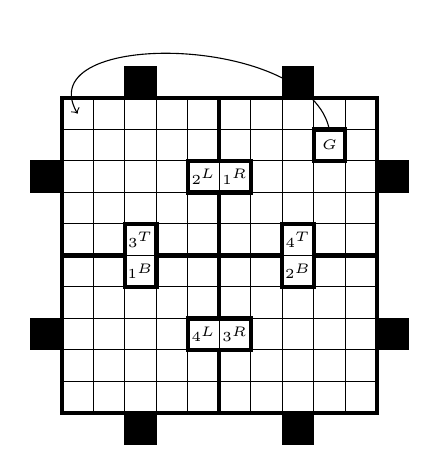
\begin{tikzpicture}
      \draw[step=0.4,thin,shift={(0.2,0.2)}] (0.8,0.8) grid (4.8,4.8);
      \draw[ultra thick] (1,1) rectangle (5,5);
      \draw[ultra thick] (3,1) -- (3,1.8);
      \draw[ultra thick] (3,2.2) -- (3,3.8);
      \draw[ultra thick] (3,4.2) -- (3,5);
      \draw[ultra thick] (1,3) -- (1.8,3);
      \draw[ultra thick] (2.2,3) -- (3.8,3);
      \draw[ultra thick] (4.2,3) -- (5,3);

      \draw[fill] (0.6,1.8) rectangle (1,2.2);
      \draw[fill] (0.6,3.8) rectangle (1,4.2);
      \draw[fill] (1.8,5) rectangle (2.2,5.4);
      \draw[fill] (1.8,0.6) rectangle (2.2,1);
      \draw[fill] (3.8,0.6) rectangle (4.2,1);
      \draw[fill] (5,1.8) rectangle (5.4,2.2);
      \draw[fill] (5,3.8) rectangle (5.4,4.2);
      \draw[fill] (3.8,5) rectangle (4.2,5.4);

      \draw[ultra thick] (4.2,4.2) rectangle (4.6,4.6);
      \draw[ultra thick] (3.8,2.6) rectangle (4.2,3.4);
      \draw[ultra thick] (1.8,2.6) rectangle (2.2,3.4);
      \draw[ultra thick] (2.6,3.8) rectangle (3.4,4.2);
      \draw[ultra thick] (2.6,1.8) rectangle (3.4,2.2);

      \node (R) at (1.2,4.8) {} ;
      \node (G) at (4.4,4.4) {\tiny $G$};
      \node at (2,3.2) {\tiny $3^T$};
      \node at (2,2.8) {\tiny $1^B$};
      \node at (4,3.2) {\tiny $4^T$};
      \node at (4,2.8) {\tiny $2^B$};
      \node at (2.8,4) {\tiny $2^L$};
      \node at (2.8,2) {\tiny $4^L$};
      \node at (3.2,4) {\tiny $1^R$};
      \node at (3.2,2) {\tiny $3^R$};

    %   \draw[step=0.4,thin,shift={(0.2,0)}] (8.799,1.999) grid (10.8,4);
    %   \draw[ultra thick] (9,3.2) -- (8.6,3.2) -- (8.6,2.8) -- (9,2.8) -- (9,2) -- (9.8,2);
    %   \draw[ultra thick] (9,3.2) -- (9,4) -- (9.8,4) -- (9.8,4.4) -- (10.2,4.4) -- (10.2,4);
    %   \draw[ultra thick] (10.2,4) -- (11,4) -- (11,3.2) -- (11.4,3.2) -- (11.4,2.8) -- (11,2.8);
    %   \draw[ultra thick] (9.8,2) -- (9.8,1.6) -- (10.2,1.6) -- (10.2,2) -- (11,2) -- (11,2.8);
    %   \draw[ultra thick] (10.2,3.2) rectangle (10.6,3.6);

    %   \node at (10.4,3.4) {\small $G$};
    %   \node at (8.8,3)    {\small $L$};
    %   \node at (11.2,3)   {\small $R$};
    %   \node at (10,1.8)   {\small $B$};
    %   \node at (10,4.2)   {\small $T$};

    %   \node at (3,0.7) {\Large a)};
    %   \node at (10,0.7) {\Large b)};

      \draw [->] (G.north) to [out=100,in=120] (R.center);
    \end{tikzpicture}
  \end{adjustbox}